\documentclass[10pt]{article}
\usepackage[pdftex]{graphicx, color}
\usepackage{listings}
\usepackage{amsmath}
\usepackage{amsfonts}
\usepackage{amssymb}
\usepackage{mathtools} 
\usepackage{tikz}
\usepackage{qtree}
\usepackage{hyperref}
\usepackage{ulem}
\usepackage{seqsplit}
\usetikzlibrary{automata,positioning}

\headheight 8pt \headsep 20pt \footskip 30pt
\textheight 9in \textwidth 6.5in
\oddsidemargin 0in \evensidemargin 0in
\topmargin -.35in

\newcommand {\pts}[1]{({\bf #1 pts})}
\newcommand {\response}{{\color{blue}\textbf{RESPONSE:}\\}}

\lstset{basicstyle=\small\ttfamily,breaklines=true}

\begin{document}


\begin{center}
	\Large CS131 Compilers: Writing Assignment 1\\Due 11:59pm March 12, 2023
\end{center}



\begin{center}
	%% Change this:
	\LARGE Name - ID
\end{center}




\begin{center}
	%% Change this:
	I worked with Name1 Name2 ...
	\small \\Complteted on \today
\end{center}

\begin{center}
	\large \textbf{Code of Conduct}    \\
\end{center}

\small \textbf{This writing assignments should be your own individual work. Discussion on concept, methodology, and class materials are welcomed, but you should list all the people you have discussed with. Copying is strictly prohibited. Plagiarism, once confirmed, may result in assignment grades reduced to zero for all involved people. And this event will be reported. Also you should use \LaTeX \ to produce your response based on this template. Submission in other forms won't be graded.  }


\begin{figure}[h]
	\centering
	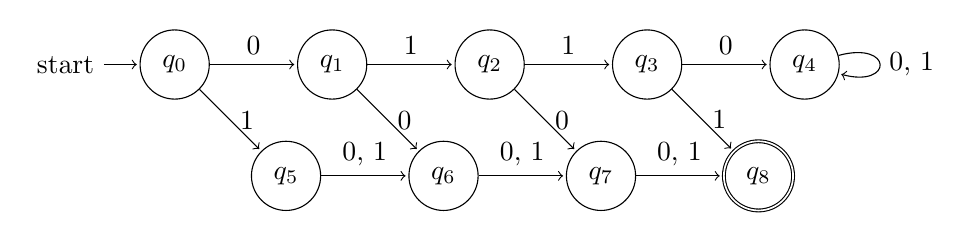
\begin{tikzpicture}[shorten >=1pt,node distance=2cm,on grid,auto]
		\node[state, initial] (q_0) {$q_0$};
		\node[state] (q_1) [right=of q_0] {$q_1$};
		\node[state] (q_2) [right=of q_1] {$q_2$};
		\node[state] (q_3) [right=of q_2] {$q_3$};
		\node[state] (q_4) [right=of q_3] {$q_4$};
		\node[state] (q_5) [below right=of q_0] {$q_5$};
		\node[state] (q_6) [below right=of q_1] {$q_6$};
		\node[state] (q_7) [below right=of q_2] {$q_7$};
		\node[state, accepting] (q_8) [below right=of q_3] {$q_8$};
		\path[->]
		(q_0) edge node [above]{0} (q_1)
		edge node [right]{1} (q_5)
		(q_1) edge node [above]{1} (q_2)
		edge node [right]{0} (q_6)
		(q_2) edge node [above]{1} (q_3)
		edge node [right]{0} (q_7)
		(q_3) edge node [above]{0} (q_4)
		edge node [right]{1} (q_8)
		(q_4) edge [loop right] node {0, 1} (q_4)
		(q_5) edge node [above]{0, 1} (q_6)
		(q_6) edge node [above]{0, 1} (q_7)
		(q_7) edge node [above]{0, 1} (q_8);
	\end{tikzpicture}
	\caption{Automata Drawn by Tikz package}
	\label{fig:tikz0}
\end{figure}

\begin{figure}[h]
	\centering
	\begin{center}
		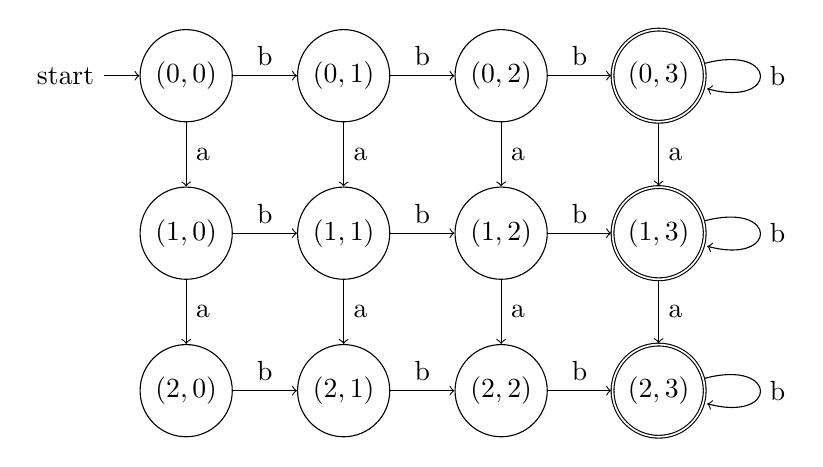
\begin{tikzpicture}
			%\draw [help lines] (-1,1) grid (8,-6);
			\node[state,initial] (11) at(0,0) {$(0,0)$};
			\node[state] (12) at(2,0) {$(0,1)$};
			\node[state] (13) at(4,0) {$(0,2)$};
			\node[state,accepting] (14) at(6,0) {$(0,3)$};
			\node[state] (21) at(0,-2) {$(1,0)$};
			\node[state] (22) at(2,-2) {$(1,1)$};
			\node[state] (23) at(4,-2) {$(1,2)$};
			\node[state,accepting] (24) at(6,-2) {$(1,3)$};
			\node[state] (31) at(0,-4) {$(2,0)$};
			\node[state] (32) at(2,-4) {$(2,1)$};
			\node[state] (33) at(4,-4) {$(2,2)$};
			\node[state,accepting] (34) at(6,-4) {$(2,3)$};
			
			\path[->] (11) edge[right] node{a} (21);
			\path[->] (12) edge[right] node{a} (22);
			\path[->] (13) edge[right] node{a} (23);
			\path[->] (14) edge[right] node{a} (24);
			\path[->] (21) edge[right] node{a} (31);
			\path[->] (22) edge[right] node{a} (32);
			\path[->] (23) edge[right] node{a} (33);
			\path[->] (24) edge[right] node{a} (34);
			\path[->] (11) edge[above] node{b} (12);
			\path[->] (12) edge[above] node{b} (13);
			\path[->] (13) edge[above] node{b} (14);
			\path[->] (21) edge[above] node{b} (22);
			\path[->] (22) edge[above] node{b} (23);
			\path[->] (23) edge[above] node{b} (24);
			\path[->] (31) edge[above] node{b} (32);
			\path[->] (32) edge[above] node{b} (33);
			\path[->] (33) edge[above] node{b} (34);
			\path[->] (14) edge[right,loop right] node{b} (14);
			\path[->] (24) edge[right,loop right] node{b} (24);
			\path[->] (34) edge[right,loop right] node{b} (34);
		\end{tikzpicture}
	\end{center}
	\caption{Automata drawn by Tikz package}
	\label{fig:tikz1}
\end{figure}

\begin{figure}[h]
	{\Tree [.. [.. [.a ][.* [.+ [.b ][.c ]] ] ][.\# ]]}
	\caption{Tree drawn by Tikz-qtree package}
	\label{fig:tikz2}
\end{figure}
\newpage
\begin{enumerate}
	\item \pts{$4\times1 = 4$} For each of the follow prompts, write any non-empty sentence:
	      \begin{enumerate}
	      	\item Name one reason why you would like to sign up this class.\\\response
	      	\item Name one of your biggest concerns or difficulties about this class.\\\response
	      	\item How will you schedule your time to complete this course successfully?\\\response
	      	\item Do you read the Code of Conduct carefully?\\\response
	      \end{enumerate}
	\item \pts{$5\times 2=10$} Write a relevant regular expression or draw an automata(DFA/NFA/$\epsilon$-NFA) that correctly represents the regular language described each question. Your response should be sound and complete. Alphabet $\Sigma = \{0,1\}$ if not other specified.
	      \begin{enumerate}
	      	\item $L_1=\{\text{All strings that contain at \textbf{most} two 0's}\}$\\
	      	      \response 
	      	\item $L_2=\{\text{All strings that contain at \textbf{least} two 1's}\}$\\
	      	      \response
	      	\item $L_3=L_1-L_2=L_1\cap \overline {L_2}$\\
	      	      \response
	      	\item $L_4=\{\text{All strings that no sequential 000 appears}\}$\\
	      	      \response
	      	\item $L_5=\{\text{All strings that contains an even number of 0's}\}$\\
	      	      \response
	      \end{enumerate}
	      \newpage
	\item \pts{$3\times 5=15$} Use regular expression or \textbf{clear} natural language to describe the automata. You may not have learned formal methods, but you can figure it out just by your brilliant brains and observations!
	      \begin{enumerate}
	      	\item  $A_1$
	      	      \begin{figure}[h]
	      	      	\centering
	      	      	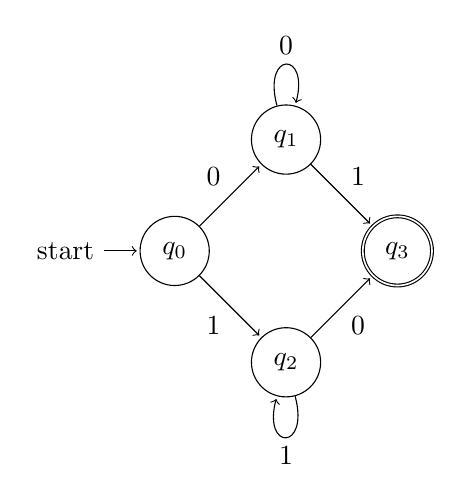
\begin{tikzpicture}[shorten >=1pt,node distance=2cm,on grid,auto] 
	      	      		\node[state,initial] (q_0)   {$q_0$}; 
	      	      		\node[state] (q_1) [above right=of q_0] {$q_1$}; 
	      	      		\node[state] (q_2) [below right=of q_0] {$q_2$}; 
	      	      		\node[state,accepting](q_3) [below right=of q_1] {$q_3$};
	      	      		\path[->] 
	      	      		(q_0) edge  node {0} (q_1)
	      	      		edge  node [swap] {1} (q_2)
	      	      		(q_1) edge  node  {1} (q_3)
	      	      		edge [loop above] node {0} ()
	      	      		(q_2) edge  node [swap] {0} (q_3) 
	      	      		edge [loop below] node {1} ();
	      	      	\end{tikzpicture}
	      	      	\caption{$A_1$}
	      	      	\label{fig:tkiza1}
	      	      \end{figure}
	      	      \\\response
	      	      \newpage \item $A_3$\begin{figure}[h]
	      	      \centering
	      	      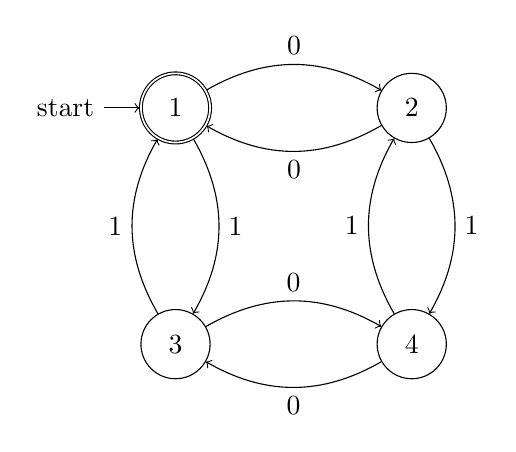
\begin{tikzpicture}
	      	      	\node[state,initial,accepting] (00) {1};
	      	      	\node[state] (01) at(3,0) {2};
	      	      	\node[state] (10) at(0,-3) {3};
	      	      	\node[state] (11) at(3,-3) {4};
	      	      			
	      	      	\path[->]
	      	      	(00) edge[bend left,above] node{0} (01)
	      	      	(01) edge[bend left,below] node{0} (00)
	      	      	(10) edge[bend left,above] node{0} (11)
	      	      	(11) edge[bend left,below] node{0} (10)
	      	      			
	      	      	(00) edge[bend left,right] node{1} (10)
	      	      	(10) edge[bend left,left] node{1} (00)
	      	      	(01) edge[bend left,right] node{1} (11)
	      	      	(11) edge[bend left,left] node{1} (01)
	      	      			
	      	      	;
	      	      \end{tikzpicture}
	      	      \caption{$A_3$}
	      	      \label{fig:tikza3}
	      	\end{figure}\\\response
	      	\newpage \item $A_2$
	      	\begin{figure}[h]
	      		\centering
	      		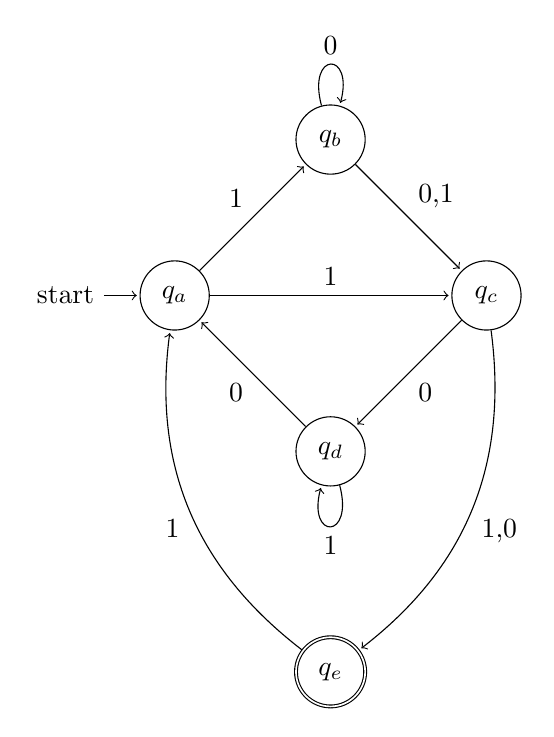
\begin{tikzpicture}[shorten >=1pt,auto,node distance=2.8cm]
	      			\node[initial,state] (A)                    {$q_a$};
	      			\node[state]         (B) [above right of=A] {$q_b$};
	      			\node[state]         (D) [below right of=A] {$q_d$};
	      			\node[state]         (C) [below right of=B] {$q_c$};
	      			\node[accepting,state]         (E) [below of=D]       {$q_e$};
	      			
	      			\path[->]          (A)  edge              node {1} (B)
	      			edge              node {1} (C)
	      			(B) edge [loop above] node {0} (B)
	      			edge              node {0,1} (C)
	      			(C) edge              node {0} (D)
	      			edge [bend left]  node {1,0} (E)
	      			(D) edge [loop below] node {1} (D)
	      			edge              node {0} (A)
	      			(E) edge [bend left]  node {1} (A);
	      		\end{tikzpicture}
	      		\caption{$A_2$}
	      		\label{fig:tkiza2}
	      	\end{figure}
	      	\\\response
	      \end{enumerate}
	      \newpage
	\item \pts{$20$} Convert the following regular expression to minimized DFA, the process is \textbf{not required}. \textbf{But showing your process may save your score} if your ultimate answer is accidentally wrong. You may spend a lot of time on these problems, since the score account is several times as those of other problems. Be focused.
	      $$00100+001(0+1)^*+010101+001^*101+101^*0+(010)^*+01(1+0^*)10$$\\(Hint: draw the $\epsilon-$NFA(NFA that allows $\epsilon$) first, and then convert it to DFA, and then run the Minimizing Algorithm) To draw your automata, you can refer to the automata examples in the preface.\\
	              
	      \begin{enumerate}
	      	\item Parse tree for regex (optional)
	      	\item NFA (optional)
	      	\item DFA (optional)
	      	\item minimized DFA (required)
	      \end{enumerate}
	      \response
\end{enumerate}
\vfill
\hrule
\center{\large\textbf{End of This Assignment}}

\end{document}